


\section{Supervised Learning: A First Approach}

\subsection{From Traditional Programming to Machine Learning}

In traditional computer science, a program is explicitly written to map inputs to outputs:

\[
\text{Data} + \text{Program} \rightarrow \text{Computer} \rightarrow \text{Output}
\]

Here, the program defines deterministic rules, such as \texttt{if-else} statements.

\vspace{1em}
Machine learning inverts this paradigm:
\[
\text{Data} + \text{Output} \rightarrow \text{Computer} \rightarrow \text{Program (Model)}
\]
The computer now learns the mapping from examples rather than explicit programming.  
The more representative the data, the better the learned model.

\begin{center}
\begin{tikzpicture}[
    node distance=2.8cm,
    process/.style={rectangle, draw, rounded corners, text centered, minimum height=1cm, minimum width=2cm, fill=blue!10},
    arrow/.style={-{Stealth[length=3mm]}, thick}
]
\node (data) [process] {Data};
\node (prog) [process, right of=data] {Program};
\node (comp) [process, right of=prog] {Computer};
\node (out) [process, right of=comp] {Output};

\draw [arrow] (data) -- (prog);
\draw [arrow] (prog) -- (comp);
\draw [arrow] (comp) -- (out);

\node [below=1.2cm of comp, align=center] (caption1)
{Traditional Programming: Rules are explicitly coded.};

\node (data2) [process, below=2cm of data] {Data};
\node (out2) [process, right of=data2] {Output};
\node (comp2) [process, right of=out2] {Computer};
\node (model) [process, right of=comp2] {Program (Model)};

\draw [arrow] (data2) -- (out2);
\draw [arrow] (out2) -- (comp2);
\draw [arrow] (comp2) -- (model);

\node [below=1.2cm of comp2, align=center] (caption2)
{Machine Learning: The computer learns the program from data.};
\end{tikzpicture}
\end{center}

\subsection{Learning from Data}

\subsubsection{Example: ECG Data}

Electrocardiogram (ECG) signals vary in time and across individuals. Each signal segment can be labeled as one of several heartbeat types:

\[
y =
\begin{cases}
\text{NA} & \text{Normal Activity}\\
\text{AF} & \text{Atrial Fibrillation}\\
\text{RB} & \text{Resting Beat}
\end{cases}
\]

The task is to learn a model that maps input signals to the correct label.

\subsubsection{Defining Learning}

An \textbf{agent} learns from experience $E$ with respect to a task $T$ and a performance measure $P$ if its performance on $T$, measured by $P$, improves with experience $E$.

\subsection{Supervised Datasets}

A supervised dataset consists of labeled examples:
\[
T = \{(x_1, y_1), (x_2, y_2), \dots, (x_n, y_n)\}
\]
where $x_i$ is a feature vector and $y_i$ is the known output.

\textbf{Examples:}
\begin{itemize}
    \item \textbf{Housing Prices:} $y_i$ = price, $x_i$ = location, size, year, etc.
    \item \textbf{Stock Prediction:} $y_i$ = up/down, $x_i$ = time-based features.
\end{itemize}

\subsection{Types of Supervised Problems}

\begin{itemize}
    \item \textbf{Binary Classification:} $y \in \{0,1\}$
    \item \textbf{Multiclass Classification:} $y \in \{1, 2, \dots, K\}$
    \item \textbf{Regression:} $y \in \mathbb{R}$
\end{itemize}

The goal is to find a function $h(x)$ that approximates $y$:
\[
h(x_i) \approx y_i, \quad \forall i = 1, \dots, n
\]

\subsection{The Hypothesis Space}

Let $\mathcal{H}$ denote the set of candidate functions (hypotheses). Each $h \in \mathcal{H}$ represents one possible model:

\[
h(x) = \beta_0 + \beta_1 x_1 + \dots + \beta_p x_p
\]

The objective is to select the hypothesis that best fits the data.

\subsection{Loss Function and Model Selection}

The \textbf{loss function} quantifies how well a hypothesis performs:

\[
L_{\text{MSE}}(h, T) = \frac{1}{n}\sum_{i=1}^{n}(h(x_i) - y_i)^2
\]
\[
L_{\text{MAE}}(h, T) = \frac{1}{n}\sum_{i=1}^{n}|h(x_i) - y_i|
\]

A perfect fit ($L=0$) may indicate overfitting — the model memorizes the training data and fails to generalize.

\subsubsection{Expected Loss}

We aim to minimize the expected loss:
\[
\mathbb{E}_{(x,y)\sim P}[L(h(x), y)]
\]
Since the population distribution $P$ is unknown, we approximate it with train/validation/test splits:
\[
80\% \text{ train}, \ 10\% \text{ validation}, \ 10\% \text{ test.}
\]

\subsubsection{No Free Lunch Theorem}
No single model works for every problem — each dataset has its own structure. Model choice must depend on the problem context.

\subsection{Supervised Learning Workflow}

\begin{center}
\begin{tikzpicture}[
    node distance=0.1cm,
    stage/.style={rectangle, draw, rounded corners, text centered, minimum height=1cm, fill=green!10, text width=3cm},
    arrow/.style={-{Stealth[length=3mm]}, thick}
]
\node (data) [stage] {Labeled Data};
\node (split) [stage, right=of data] {Train / Validation / Test Split};
\node (train) [stage, right=of split] {Model Training};
\node (validate) [stage, right=of train] {Model Validation};
\node (test) [stage, right=of validate] {Testing \& Evaluation};

\draw [arrow] (data) -- (split);
\draw [arrow] (split) -- (train);
\draw [arrow] (train) -- (validate);
\draw [arrow] (validate) -- (test);
\end{tikzpicture}
\end{center}

\subsection{Underfitting and Overfitting}

\begin{itemize}
    \item \textbf{Underfitting:} Model too simple; fails to capture structure.
    \item \textbf{Overfitting:} Model too complex; captures noise.
\end{itemize}

Balancing bias and variance is crucial for generalization.

\begin{center}
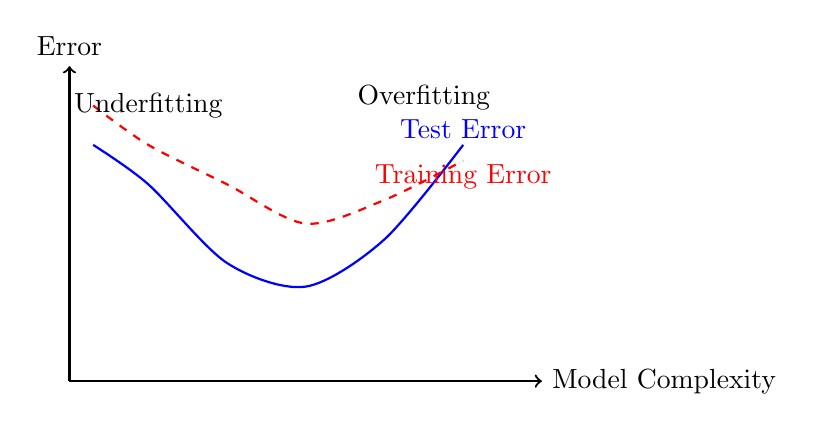
\begin{tikzpicture}[
scale=1.0, every node/.style={scale=1.0},
axis/.style={->, thick},
curve/.style={thick, smooth}
]
\draw[axis] (0,0) -- (6,0) node[right]{Model Complexity};
\draw[axis] (0,0) -- (0,4) node[above]{Error};

\draw[curve, blue] plot[smooth] coordinates {(0.3,3) (1,2.5) (2,1.5) (3,1.2) (4,1.8) (5,3)};
\draw[curve, red, dashed] plot[smooth] coordinates {(0.3,3.5) (1,3) (2,2.5) (3,2) (4,2.3) (5,2.8)};

\node[blue] at (5,3.2) {Test Error};
\node[red] at (5,2.6) {Training Error};
\node at (1,3.5) {Underfitting};
\node at (4.5,3.6) {Overfitting};
\end{tikzpicture}
\end{center}

\subsection{k-Nearest Neighbors (k-NN)}

In $k$-NN, predictions are based on the labels of the $k$ closest data points to a query $x_*$:

\[
\|x_i - x_*\| = \sqrt{\sum_{j=1}^{p}(x_{ij} - x_{*j})^2}
\]

\textbf{Hyperparameter:} $k$
\begin{itemize}
    \item Low $k$: possible overfitting.
    \item High $k$: possible underfitting.
\end{itemize}

\begin{algorithm}[H]
\SetAlgoLined
\KwIn{Training set $T = \{(x_1, y_1), \dots, (x_n, y_n)\}$, query $x_*$, number of neighbors $k$}
\KwOut{Predicted label $\hat{y}_*$}
\BlankLine
\ForEach{$(x_i, y_i) \in T$}{
    Compute distance $d_i = \|x_i - x_*\|$ (e.g., Euclidean)
}
Sort $d_i$ in ascending order\;
Select $k$ nearest neighbors\;
\eIf{classification}{
    $\hat{y}_* \leftarrow$ majority label among $k$ neighbors
}{
    $\hat{y}_* \leftarrow \frac{1}{k}\sum_{i=1}^{k} y_i$ (mean for regression)
}
\caption{k-Nearest Neighbors Algorithm}
\end{algorithm}

\subsubsection{Normalization}

Since distances depend on scale, normalize each feature:
\[
x_j' = \frac{x_j - \mu_j}{\sigma_j}
\]
where $\mu_j$ and $\sigma_j$ are the mean and standard deviation of feature $j$.

\subsection{Summary}

Supervised learning aims to infer a mapping from inputs to outputs based on labeled data.
The process involves:
\begin{enumerate}
    \item Defining the hypothesis space $\mathcal{H}$
    \item Choosing a suitable loss function $L$
    \item Optimizing $h \in \mathcal{H}$ to minimize $L$
    \item Validating and testing to ensure generalization
\end{enumerate}

A good model balances complexity and performance, avoiding both underfitting and overfitting.


